\documentclass[12pt]{article}
\usepackage[margin=1in]{geometry}
\usepackage{amsmath,amsthm,amssymb}
\usepackage{stmaryrd}
\usepackage{enumitem}
\usepackage{xspace}
\usepackage{tikz}
\usepackage{graphicx}
\graphicspath{ {./imgs/} }
\usepackage{underscore}
% \usetikzlibrary{matrix,arrows,decorations.pathmorphing,cd}
\setlist{
  listparindent=\parindent,
}
\usepackage{pgfplots}
\pgfplotsset{width=10cm,compat=1.9}
\usepackage{float}
\usepackage{polynom}
\usepackage{hyperref}
\expandafter\def\expandafter\UrlBreaks\expandafter{\UrlBreaks%  save the current one
  \do\a\do\b\do\c\do\d\do\e\do\f\do\g\do\h\do\i\do\j%
  \do\k\do\l\do\m\do\n\do\o\do\p\do\q\do\r\do\s\do\t%
  \do\u\do\v\do\w\do\x\do\y\do\z\do\A\do\B\do\C\do\D%
  \do\E\do\F\do\G\do\H\do\I\do\J\do\K\do\L\do\M\do\N%
  \do\O\do\P\do\Q\do\R\do\S\do\T\do\U\do\V\do\W\do\X%
  \do\Y\do\Z}
\newcommand{\qq}{\noindent\textbf{Q:} }
\newcommand{\N}{\mathbb{N}}
\newcommand{\Z}{\mathbb{Z}}
% various useful symbols defined here:
\newcommand{\np}{\textsc{NP}\xspace}
\newcommand{\conp}{\textsc{coNP}\xspace}
\newcommand{\p}{\textsc{P}\xspace}
\newcommand{\twosat}{\textsc{2-Sat}\xspace}
\newcommand{\threesat}{\textsc{3-Sat}\xspace}
\newcommand{\vc}{\textsc{VertexCover}\xspace}
\newcommand{\is}{\textsc{IndependentSet}\xspace}
\newcommand{\nphard}{\textsc{NP-hard}\xspace}
\newcommand{\npcomplete}{\textsc{NP-complete}\xspace}
\newsavebox{\wideeqbox}
\newenvironment{proof-idea}{\noindent{\bf Proof Idea}\hspace*{1em}}{\qed\bigskip}
\newenvironment{wideeq}
  {\begin{displaymath}\begin{lrbox}{\wideeqbox}$\displaystyle}
  {$\end{lrbox}\makebox[0pt]{\usebox{\wideeqbox}}\end{displaymath}}


\makeatletter
\renewcommand*\env@matrix[1][\arraystretch]{%
  \edef\arraystretch{#1}%
  \hskip -\arraycolsep
  \let\@ifnextchar\new@ifnextchar
  \array{*\c@MaxMatrixCols c}}
\makeatother

\newtheorem*{theorem}{Theorem}

\newtheorem*{prop}{Proposition}
\newtheorem*{conjecture}{Conjecture}

\theoremstyle{remark}
\newtheorem*{note}{Note}

\theoremstyle{remark}
\newtheorem*{remark}{Remark}

\newenvironment{must-show}{\noindent{\bf Must Show:}\hspace*{0.5em}}{\qed\bigskip}


\title{Programming Languages Theory Notes}
\author{Jae Tak Kim
}
\date{Fall 2020}

\begin{document}

\maketitle
\tableofcontents
\newpage

\section{Introduction}
\textit{Source:} Isil Dillig -- A Gentle Introduction to Program Analysis
\subsection{Overview}

\subsubsection{What is a typical static analysis question?}
Given source code of program $P$ and desired property $Q$, does $P$ exhibit $Q$ in \textit{all possible executions}?

\subsubsection{Soundness vs Completeness?}
In formal logic, an expression is sound if whenever the premise is true, the conclusion is also aways true. There's no guarantees about the conclusion if the premise is false. In the case of static analysis, the premise is that the program is unsafe and the conclusion is that our static analysis will say the program is unsafe. Thus, if the program is really unsafe, then the analysis will \textit{always} tell us that the program is unsafe. However, it's possible that the analysis will take us it's unsafe even when the program is safe.

Our analysis is complete if our program analysis always tells us the truth. Thus, completeness is a stronger condition than soundness.

\subsubsection{Describe the inherent limitations of static analysis.}
The question of trying to see if the program has a property in every single execution is undecidable. A short proof of is uses the Rice Theorem which states that all nontrivial properties are undecidable. We can even reduce this to the halting problem. 

Thus, our static analysis will be either unsound(we definitely don't want this since we don't want our analysis to say that our program is safe when it isn't), sound but incomplete($\exists$ false positives), or non-terminating(we don't want our analysis to run forever!). Clearly, the best option is the second one, so most analysis techniques will be sound but incomplete.


\subsubsection{How do you design sound static analyses?}
\begin{figure}[h]
    \centering
    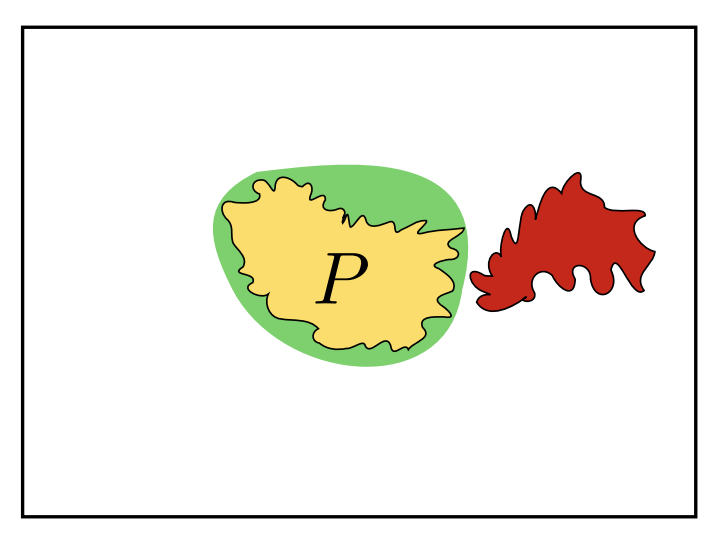
\includegraphics[scale=0.5]{overapprox}
    \caption{All possible states}
\end{figure}
We overapproximate our program behavior as little as we can. Overapproximating ensures that we never give an invalid answer. If $P$ region is the actual behavior of our program, and the green bubble is the analysis, then any states outside of the green bubble will be correctly classified. States within the green bubble but outside of the region $P$ will be false alarms (false positives). We overapproximate using abstractions so the goal of static analysis is to construct abstractions that are precise enough (few false alarms) and scale to real programs.


\subsubsection{Abstraction interpretation}
Framework for constructing sound-by-construction static analyses. Includes abstract domain, abstract function, concretization function, and abstract transformers/semantics.
\begin{figure}[h]
    \centering
    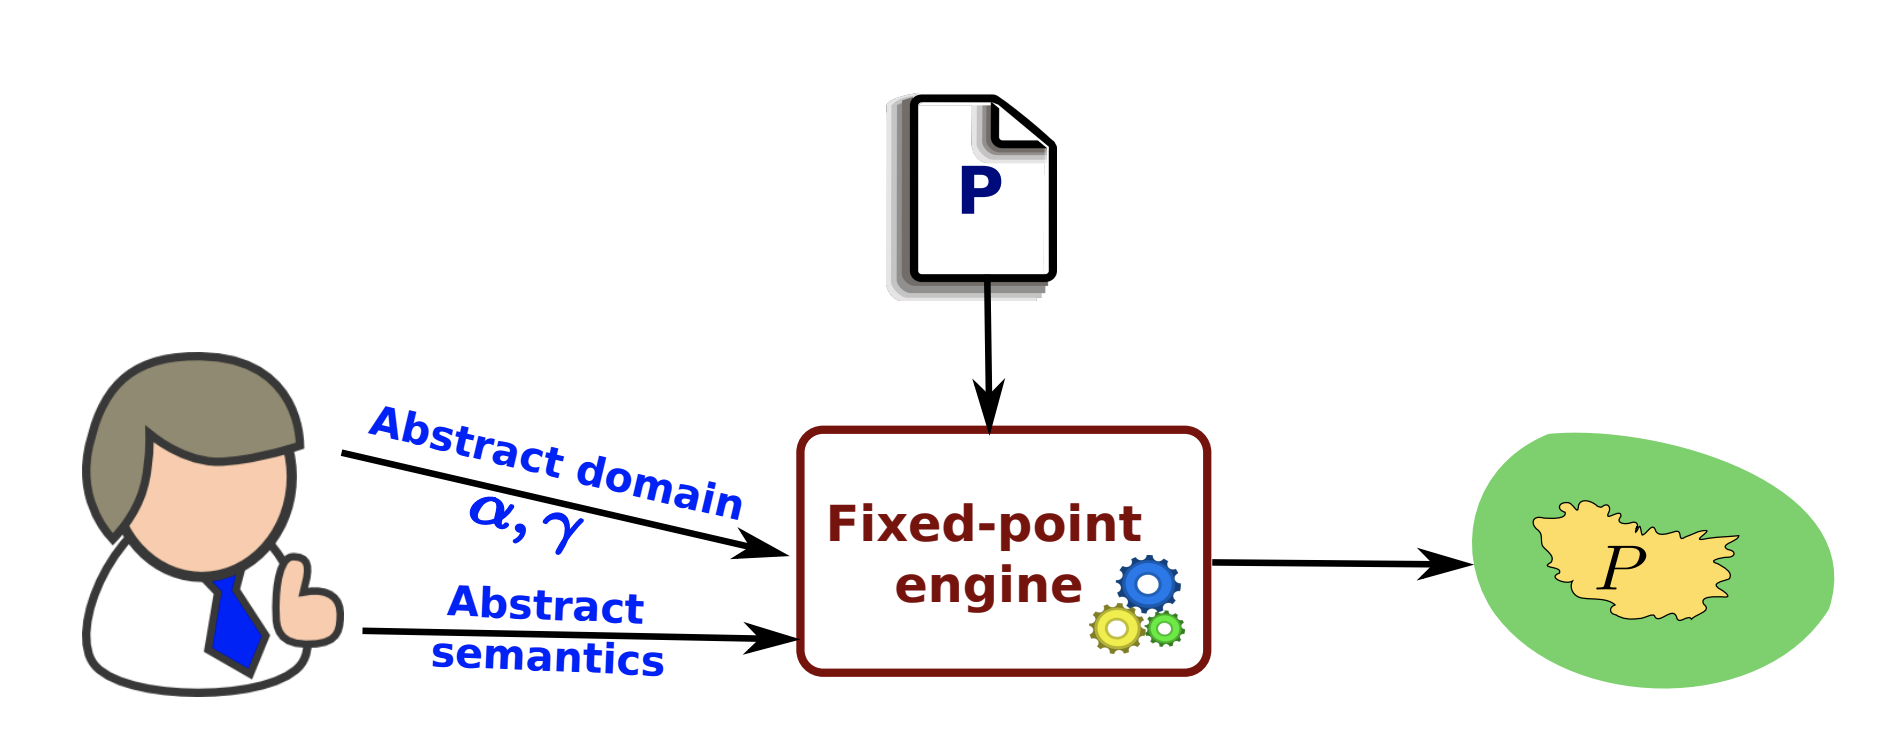
\includegraphics[scale=0.3]{analysis-process}
\end{figure}


\subsubsection{What is the idea of least-fixed point in a fixed-point computation?}
You start with an underapproximation and grow the approximation until it stops growing. This is the point where your analysis is as precise as it can be while still being sound.
\begin{figure}[h]
    \centering
    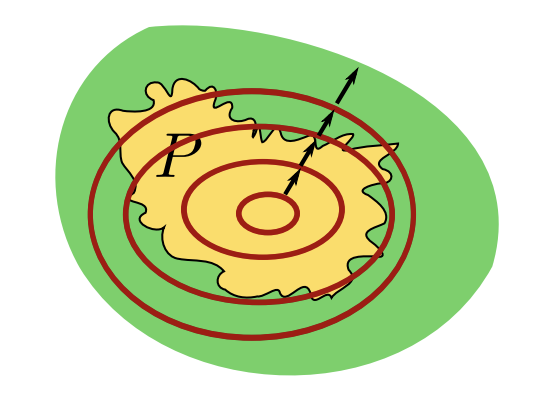
\includegraphics[scale=0.5]{least-fixed-point.png}
\end{figure}

\section{Lattice Theory}
\subsubsection{Define Lattice and Fixed-points}

\subsubsection{Define a monotone function on a lattice + intuition}
A function $f: L \to L$ is \textbf{monotone} if $\forall x,y \in L$, $x \sqsubseteq y \Rightarrow f(x) \sqsubseteq f(y)$. A monotonic function preserves partial ordering. Also can be thought of as ``increasing the input also increases output.'' Note that this is not the same thing as extensive. A function $f$ is \textbf{extensive} if $\forall x \in L, x \sqsubseteq f(x)$.

We can think of a monotone function as a function where more precise input cannot lead to less precise output.

\subsection{Equations and Fixed-Points}
\subsubsection{What is the fixed-point theorem and the general idea of the proof?}
\begin{theorem}
    In a lattice $L$ with finite height, every monotone function $f$ has a unique least fixed-point given by
    \[fix(f) = \bigsqcup_{i \geq 0} f^i (\bot)\]
\end{theorem}
\begin{proof-idea}
Because $\bot$ is the unique smallest element, we can get a chain of inclusions. Since the lattice is of finite height, it must stop somewhere, and this shows that for some $i$, $f^i(\bot) \sqsubseteq f^{i+1}(\bot)$, making this a fixed-point. We can make an argument with a least fixed-point $x$ that because $\bot \sqsubseteq x$, $f^i(\bot) \sqsubseteq x$ as well, showing that this is indeed the least fixed-point. It is unique by the fact that the partial order relation is anti-symmetric.
\end{proof-idea}

% \begin{enumerate}
%     \item What is a typical static analysis question?
%     \item Soundness vs Completeness?
%     \item Describe the inherent limitations of static analysis.
%     \item How do you design sound static analyses?
% \end{enumerate}

\section{Context-Sensitive Data-Dependence Analysis via LCL-Reachability}
\begin{enumerate}
  \item What is the basic idea of CFL Reachability and why is it better/different than the usual static analyses methods? [CFLR]
  
  The idea is that this is just another framework to perform static analysis. Instead of the abstract interpretation/least-fixed-points framework, this one turns the problem into a graph reachability problem. The first step is to get to an ordinary graph reachability problem where each node in the CFG tells you the correct element of the abstract domain by considering the union of values that can be reached by the graph from (start\_main, bot). While this would get you something similar to using abstract interpretation, CFL-Reachability goes one step further and considers only paths that can be reached through paths that create words that are in a particular grammar. The example in the paper defines realizable paths, which are paths that are possible executions of the program (though it also includes non-executable ones). Thus, the analysis gives you a tighter and more precise analysis than what you might otherwise get.
  \item How does LCL improve on CFL Reachability and how is it different?
  \item What is data-dependence condition? Further, what is structure-transmitted data dependence? How are context-sensitivity and data-dependence represented as a CFL?
  \item Why is the LCL-R algorithm given only an approximation alg instead of an exact one?
  
  Because "a precise analysis that simultaneously captures two or more well-balanced properties is undecidable" (Reps undeciability of CSDD-A)

  \item What does Trellis automata have to do with anything?
  
  They are the automata/operational form of LCL which are more readable than the grammar version.

  \item What is the motivating example?
  \item How is LCL-Reachability defined?
  
  One main thing is to show the equivalence of LCL-Reachability with context-sensitive data-dependent analysis. You do this by showing that you can construct a graph in a way that LCL-reachability between two points in the program means that the concatenation of the edge labels in the path are elements from the inter-Dyck language (which in itself must correspond to context-sensitivity and data-dependence). Since LCL grammars are hard to work with, we use trellis automatons instead, and show that a certain kind of trellis automata, the GWTA $\subseteq$ STA $\subseteq$ TA, accepts the inter-Dyck language. But it turns out that constructing TA's are difficult as well as proving things about them so instead, we construct a DSTM for $\mathbb{D}_{mn}$ and then show a way to convert this DSTM into $K_{\mathbb{D}_{mn}}$.

  Only after showing this construction and its correctness can we get to the actual algorithm for LCL-reachability, first shown with HTAs and then with GWTAs in particular.

  \item Where does the approximation come in for LCL-reachability algorithm?
  \item What is the main idea of the LCL-reachability algorithm?
  \item What's the difference between HTA and GWTA?
  
  The reason we needed a GWTA instead of an HTA was because the constructive proof from HTA to DSTM and vice versa was wrong. To correct for this, we need to use a STA, more specifically a GWTA instead. However, this is okay as it is shown that $L(HTA) = L(STA)$ and therefore $L(DSTM) = L(HTA)$.

  Likewise, the baseline LCL-reachability algorithm is based on HTAs.

  \item Why use a GWTA instead of a HTA in the first place?
  
  The DTSM $\Rightarrow$ HTA construction in (Ibarra, Kim) was flawed because they didn't consider the fact that end-of-right-to-left (EOR) transitions are not total. For the $\mathbb{D}_{mn}$ example, the only valid states that start the left-to-right sweep again for the state at EOR transition are $q_1$ and $q_2$. This is because the states $\llparenthesis_i$ and $\llbracket_i$ at EOR indicates that no match for the right parenthesis and bracket was not found, hence the DSTM stops and rejects the string. The HTA construction did not consider this and has no mechanism to reject. Hence, what's needed is to shrink the domain set of state for the EOR representing transitions to the valid set $\{q_1, q_2\}$ instead. However, this isn't possible with HTAs, hence the need for a STA to allow for different transitions on differently labeled nodes. Since we only need two kinds of nodes, a GWTA suffices.

  \item Describe a DSTM.
  
  It's like an oblivious TM in that it's on-line, with the additional restriction that on the left-to-right sweeps, the machine can't change states or the worktape. It consists of reading a single input character at a time when it hits the leftmost blank symbol and work is only done on the right-to-left sweep.

  \item What are the additions we need to make to go from the DSTM for $D_m$ to $\mathbb{D}_{mn}$?
  
  Initially, I just thought that from the right-to-left sweep after reading in $\rrparenthesis_i$ would just need to ignore any $\llbracket_j$ until the first left parenthesis it hits is $\llparenthesis_i$. However, this doesn't work because the input $x=\llparenthesis_0 \llbracket_0 \rrparenthesis_0$ would be accepted as the DSTM would go into the accept state $q_2$ before hitting $\$$ and accepting. Thus, the DSTM for $\mathbb{D}_{mn}$ needs to consider the state where it clearly isn't done (there's still left brackets to process) while only ignoring the left brackets (or vice versa). This is accomplished through the states $q_1 \llparenthesis_i$ and $q_1 \llbracket_i$.

  Proof of correctness follows the usual for TMs, showing that the language recognized by the TM is equivalent to $\mathbb{D}_{mn}$ in both directions.
\end{enumerate}

\begin{enumerate}
  \item This thing about the cubic bottleneck. More about it + general explanation + pointers to resources?
  \item You could in theory get a nonapproximate answer right by creating a DWTA for every single path from $u$ to $v$?
\end{enumerate}

\end{document}